\section{Desenvolvimento Experimental}
\subsection{Materiais e Métodos}
Foi utilizado para o experimento o equipamento PASCO Modelo AP-8210 cosntituido por: 
\begin{itemize}
	\item Câmara  para visualização das gotas graduada em 0,1mm e com placas metálicas em seus terminais;
	\item Anéis para regulagem do foco;
	\item Lâmpada de halogênio;
	\item Filamento de fibra óptica;
	\item Termístor;
	\item Interruptor para controlar o campo elétrico da câmara
	\item Óleo de densidade 886 kg/m³.
\end{itemize}

A plataforma deve ser ligada à uma fonte de 500 V em corrente contínua, um multímetro aos terminais de seu termistor e a lâmpada a uma tensão de 12 V DC. Então, se desmonta a câmara para limpeza de sua base com um papel de pequena gramatura, remontando-a novamente. Insere-se a fibra óptica à câmara para regulagem do foco a partir dos aneis sobre a ocular. Por último, borrifa-se o óleo na câmara, fechando-a a partir de uma alavanca em sua lateral. Com o interruptor é possivel ligar o campo entre as placas metálicas.      

\subsection{Dados Obtidos Experimentalmente}
Após a realização do experimento duas vezes, foram obtidos diversos tempos de subida e descida, utilizando os mesmos, foram calculadas as velocidades de subida e descida e também o raio de cada gota, como é possível ver na tabela \ref{tab:Vel}

\begin{table}[ht!]
\centering

\begin{tabular}{l|ll|ll|ll|}
\rowcolor[HTML]{C0C0C0} 
Gota & $V_d \times 10^{-5}(m/s)$ & $\Delta V_d (m/s)$ & $V_s \times 10^{-5}(m/s)$ & $\Delta V_s (m/s)$ & $a \times 10^{-7}(m)$ & $\Delta a(m)$ \\
1    & 2,28                      & 0,01               & 2,03                      & 0,05               & 4,69                  & 0,03          \\
\rowcolor[HTML]{C0C0C0} 
2    & 2,75                      & 0,14               & 2,6                       & 0,2                & 5,16                  & 0,15          \\
3    & 2,8                       & 0,15               & 1,9                       & 0,01               & 5,21                  & 0,16          \\
\rowcolor[HTML]{C0C0C0} 
4    & 3,08                      & 0,22               & 3,1                       & 0,33               & 5,46                  & 0,23          \\
5    & 3,25                      & 0,27               & 3,39                      & 0,41               & 5,61                  & 0,27          \\
\rowcolor[HTML]{C0C0C0} 
6    & 2,06                      & 0,05               & 1,64                      & 0,06               & 4,46                  & 0,04          \\
7    & 1,43                      & 0,22               & 0,6                       & 0,33               & 3,68                  & 0,24          \\
\rowcolor[HTML]{C0C0C0} 
8    & 1                         & 0,33               & 0,91                      & 0,25               & 3,09                  & 0,4           \\
9    & 1,52                      & 0,19               & 1,5                       & 0,09               & 3,82                  & 0,21          \\
\rowcolor[HTML]{C0C0C0} 
10   & 1,65                      & 0,16               & 0,53                      & 0,35               & 3,98                  & 0,17          \\
11   & 2,1                       & 0,04               & 0,87                      & 0,26               & 4,5                   & 0,03          \\
\rowcolor[HTML]{C0C0C0} 
12   & 2,02                      & 0,06               & 1,89                      & 0,01               & 4,41                  & 0,05          \\
13   & 2,46                      & 0,06               & 1,93                      & 0,02               & 4,87                  & 0,07          \\
\rowcolor[HTML]{C0C0C0} 
14   & 3,06                      & 0,22               & 3                         & 0,31               & 5,44                  & 0,22           \\ \hline 
\end{tabular}
\caption{Valores calculados para as velocidades de descida($V_d$), velocidade de subida($V_s$) e o raio de cada gota($a$), assim como o desvio padrão associado a cada medida.}
\label{tab:Vel}
\end{table}

Com os valores obtidos e  utilizando a equação[CITAS A LA DE CIMA] é possível encontrar o valor de carga que cada gota possui, explicito na tabela \ref{tab:Car}.

\begin{table}[!htb]
\centering

\begin{tabular}{|l|ll|}
\hline
\rowcolor[HTML]{C0C0C0} 
Gota & $Carga \times 10^{-19} (C)$ & $\Delta Carga \times 10^{-19} (C)$ \\ \hline
1    & 1,09                        & 0,29                               \\ \hline
\rowcolor[HTML]{C0C0C0} 
2    & 1,49                        & 0,4                                \\ \hline
3    & 1,32                        & 0,35                               \\ \hline
\rowcolor[HTML]{C0C0C0} 
4    & 1,82                        & 0,49                               \\ \hline
5    & 2,01                        & 0,54                               \\ \hline
\rowcolor[HTML]{C0C0C0} 
6    & 0,89                        & 0,24                               \\ \hline
7    & 0,4                         & 0,11                               \\ \hline
\rowcolor[HTML]{C0C0C0} 
8    & 0,31                        & 0,08                               \\ \hline
9    & 0,62                        & 0,17                               \\ \hline
\rowcolor[HTML]{C0C0C0} 
10   & 0,46                        & 0,12                               \\ \hline
11   & 0,72                        & 0,19                               \\ \hline
\rowcolor[HTML]{C0C0C0} 
12   & 0,93                        & 0,25                               \\ \hline
13   & 1,15                        & 0,31                               \\ \hline
\rowcolor[HTML]{C0C0C0} 
14   & 1,78                        & 0,48                               \\ \hline
\end{tabular}
\caption{Valores da carga associada a cada gota, assim como o seu respectivo desvio padrão.}
\label{tab:Car}
\end{table}



\subsection{Interpretação dos Resultados}
Utilizando os dados contidos na tabela \ref{tab:Car} é possível produzir o gráfico \ref{im:Car} que contêm a carga pelo número da gota, e assim analisar de forma adequada os dados obtidos.

\begin{figure}[!htb]
	\centering
		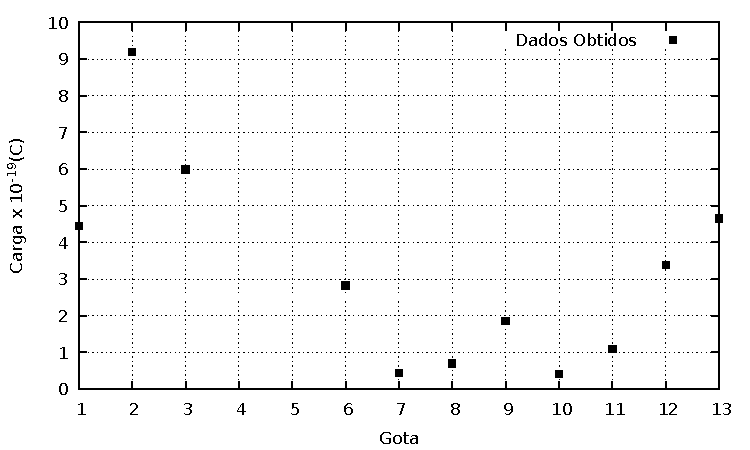
\includegraphics[scale= 1]{grafico/gotas.pdf}
	\caption{Distribuição de carga das gotas}
	\label{im:Car}
\end{figure}


Analisando o gráfico \ref{im:Car} temos que as gotas estão separadas em três grupos, um primeiro com as gotas 6,7,8,9,10,11,12, o segundo grupo com as gotas 1,2,3,4,13,14 e um terceiro grupo com a gota 5. Com isto somos levados a crer que o incremento de carga não é continuo e sim discreto ou quantizado, e isto pode ser aferido realizando a diferença entre as médias de carga de cada grupo.


